\section{Automatic Movement Overhaul}\label{sec:automatic-movement-overhaul}

As pointed out in section~\ref{subsec:problems-with-automatic-movement}, the current automatic movement method was
built as temporary means to navigate between saved bookmarks.
The method applies a linear interpolation to transition smoothly between the origin and target position leading to
movement in a straight line between the two points.
Additionally, a linear interpolation between the origin and target orientation is used to rotate the observer into the
target orientation.
While this is the easiest, and most straightforward way to smoothly move the observer through the simulation without
breaking continuity by teleporting the user, the simultaneous translation and rotation have been found to induce
disorientation followed up by motion sickness symptoms by the user.

In this section a new automatic navigation for CosmoScout is presented, which aims to make the automatic navigation
more accessible and less sickness inducing.
As parts of the navigation have not been fully implemented, we first present the concepts how the automatic
navigation system should move the observer.
After the concept, key features of the implemented solutions are presented and explained.


\subsection{Automatic Movement Concept}\label{subsec:automatic-movement-concept}

The main goal, found to reduce cybersickness for automatic movement, is reducing the complexity of the movement by
decoupling the rotation from the translation.
This way the movements are easier to read, and the user should be able to better anticipate the observers movements,
reducing motion sickness symptoms.

First, the linear interpolation is exchanged for movement along a spline.
This way, it does not change the linear movement between points in space as it was implemented before, while still
accomodating for different, non-linear paths the observer can take.
Additionally, this change is made to facilitate more variability for later development, like programmed virtual tours
along points of interest.
Additionally, the change to splines is made to enable easier collision handling for the navigation method, as
additional control points can be inserted to handle collisions and divert the movement path.

Since the origin and target location and orientation of the automatic navigation can be arbitrary points anywhere in
the simulation (both bookmarked and calculated intermediate locations), the first step is to classify the possible
locations into groups.
We propose the classification of locations based on their location relative to other bodies, and the SPICE reference
frame the location is in:
\begin{itemize}
    \item Surface locations, that are close to, or on the surface of a body, where the location's position and
    orientation are in the respective body's SPICE frame relative to the body's center;
    \item Orbit locations, where the location is not on or close to the surface, but the position and orientation
    are still relative to the body's SPICE frame and center;
    \item Interplanetary locations, where the location's position and orientation is not relative to another body's
    SPICE frame and center, but the solar system's barycenter, i.e.\ the "J2000" SPICE frame.
\end{itemize}
Through the classification of locations a set of general movements and transitions can be derived to access all of
those locations in a manner that is predictable for the user, while still general enough to minimize special cases
that could lead to unwanted behaviour.

The classification of locations leads to 3 types of movement and the transitions between them, resulting in the states
shown in figure~\ref{fig:nav-states}.

\begin{figure}[h]
    \centering
    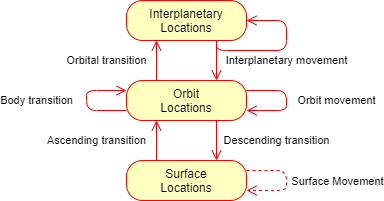
\includegraphics[width=0.5\textwidth]{content/4_3_autoNavigation/img/NavigationLocationStates}
    \caption{State diagram for the different types of locations, and the movements and transitions between them.}
    \label{fig:nav-states}
\end{figure}

The different movements are structured in layers, therefore a transition from surface to interplanetary space and
vice versa is done via transition from surface to orbit, and from orbit to interplanetary space.
Additionally, there is no explicit transition from interplanetary movement to orbital movement since the interplanetary
movements end in a position where either the destination is reached, or the observer is in a position in the target
orbit and is able to resume orbital movement immediately.

An example for this layered travel is a movement from a location on the origin body's surface to a location on the
target body's surface:
the movement starts in the "Surface movement" state, since the origin location is on a body's surface.
First, the observer transitions from the surface location to an orbit location via the ascension transition, because
the observer is still in the origin's SPICE frame.
Then, since the observer is still in the wrong frame, the observer transitions to a position for interplanetary
movement, and moves to towards the target via interplanetary movement, ending in an orbital location in the target
frame.
Then, an orbital movement is performed to move above the final location on the surface.
Finally, the observer enters a decension transitions to the final location on the surface.

While a SPICE frame is merely a nested oriented frame of reference, and therefore not limited in distance from its
center, in the context of the navigation concept, the frame is used as a general reference to a body's sphere of
influence, where the observer is eiter on the surface or in an arbitrarily, but reasonably high orbit around the body.

\subsubsection{Surface Movement}\label{subsubsec:surface-movements}

\begin{wrapfigure}{o}{0.25\textwidth}
    \centering
    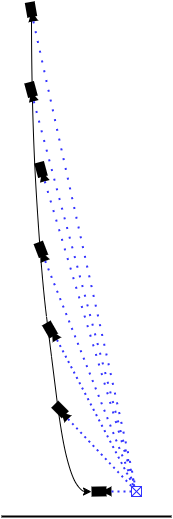
\includegraphics[width=0.1\textwidth]{content/4_3_autoNavigation/img/PlannedLanding}
    \caption{Planned automatic movement descending onto a body's surface.}
    \label{fig:new-auto-nav-descend}
\end{wrapfigure}

In this overhaul, we did not primarily focus on a solution for automatic movement on the surface of a body, since
those movements are strongly dependent on distance and topology between the target and origin.
Additionally, surface navigation is difficult to test under the current circumstances, since a connection to the DLR
map server is needed to poll street level elevation data and textures, and both were unavailable in the remote work
setting due to the COVID-19 pandemic.
In order to find a general solution, independent of distance and topology, we chose to facilitate surface movements
via orbital travel, i.e.\ transitioning from the surface origin location into orbit, using orbital movement to go to an
orbital location above the target surface location and transitioning back down to the surface at the target location.
While this solution may be inconvenient for short distances relative to the body's circumference, we assume this form
of movement to be a default solution independent of topology or distance.
Further solutions for surface movements, especially for short distances, should be easily implementable in later
works using the established framework we develop here.

The important changes in the surface movement are the transitions between surface and orbit (the landing and
ascending movements).
In order to prevent the change of reference frame, as pointed out in
section~\ref{subsec:problems-with-automatic-movement}, we plan to change the linear path and simultaneous rotation
shown in figure~\ref{fig:old-auto-nav-descend}, to a parabolic curve, so the observer's movements are always
perceived as forward, not downward, and the observer swoops into the target location on the surface, as depicted in
figure~\ref{fig:new-auto-nav-descend}.
To ease the rotation and enable the user to predict the movement, the center of the viewport is aimed at a point
slightly in front of the final position in direction of the final orientation.
This essentially separates the translation from the rotation due to the steepness of the movement.
The bulk of the rotation during the movement is at the end of the curve where the curvature is highest.

The ascending transition is basically similar, but in reverse, so the observer zooms out moving backwards and
focusing on the point of origin until it reaches the default orbital distance where the point of origin should almost
coincide with the body's center.

\subsubsection{Orbital Movement}\label{subsubsec:orbital-movements}

The default orbital distance for each body is relative to the body size, so that the orbited body always occupies the
same space of the viewport, independent of the body's size.
In order to prevent movements through the body as shown in figure~\ref{fig:old-auto-nav-collision} in
section~\ref{subsec:problems-with-automatic-movement}, we plan to use the flexibility of splines to move the observer
in circular curves around the body, while focusing the center of the viewport on the center of the body.

While this movement has simultaneous translation and rotation, this movement is not perceived by most users as the
observer moving around the body, but a rotation of the whole simulation around the body where the viewport is focused
on.
In case either the starting point, or the final location are not equidistant to the boday's center, the curve becomes
less circular, but the nature of the spline should compensate for different distances to the center automatically,
leading to the user perceiving the change in distance as the observer zooming out, away from the body during the
rotation.

For the transition from orbital to interplanetary movement, a few steps are added to reduce surprising rotations and
make the movement easier to predict by the user.

\begin{figure}[h]
    \centering
    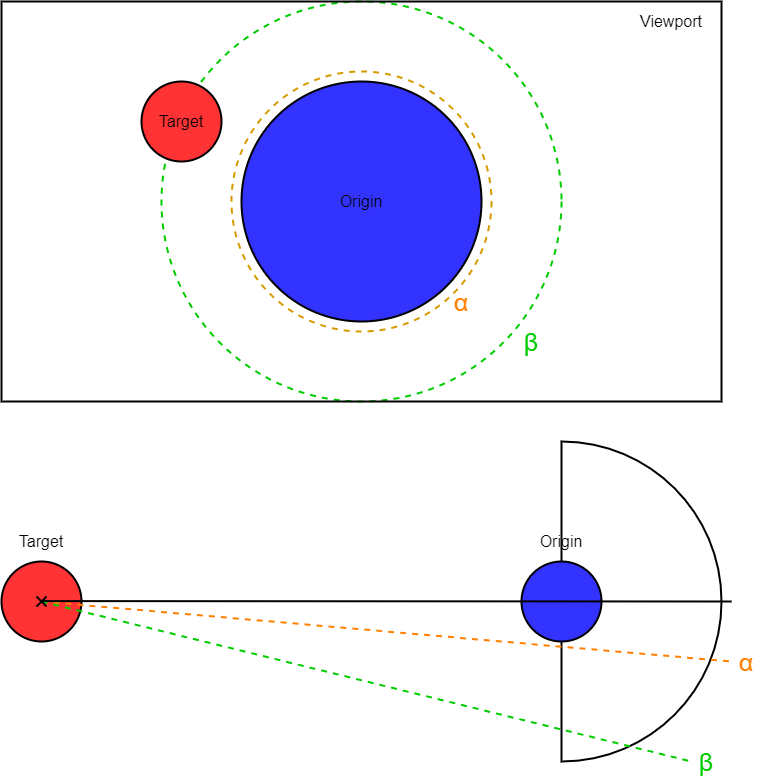
\includegraphics[width=0.66\textwidth]{content/4_3_autoNavigation/img/OrbitTransitionAngles}
    \caption{Minimum ($\alpha$) and maximum ($\beta$) angle for the transition into interplanetary movement.}
    \label{fig:orbital-transition-angles}
\end{figure}

First, the observer finds the closest suitable location where the following conditions are met:
\begin{itemize}
    \item The angle $\theta$ between the vector from the target's center to the observer, and the vector from the
    target's center to the origin's center is between the minimum allowed angle $\alpha$ and the maximum allowed
    angle $\beta$.
    \begin{equation}
        \label{eq:orbital-angles}
        \alpha \geq \theta \geq \beta
    \end{equation}

    \item The vector $\vec{v}$ between the target's center, and the observer must be longer than the vector $\vec{w}$
    between the target's center, and the origin's center.
    \begin{equation}
        \label{eq:orbital-magnitudes}
        \left\| \vec{v} \right\| > \left\| \vec{w} \right\|
    \end{equation}
\end{itemize}
The requirements are visualised in figure~\ref{fig:orbital-transition-angles}.
The first requirement (equation~\ref{eq:orbital-angles}), creates two cones from the target's center towards the origin.
The $\alpha$-cone is the minimum angle, that prevents the target from being mostly obscured by the origin body, and
the $\beta$-cone is the maximum angle, that ensures the Target is still visible on the viewport.
Both cones intersect the sphere of the origin's possible orbit locations twice, resulting in two spherical segments.
The second requirement excludes the spherical segment that is in between the origin and target bodies.
The spherical zone of the remaining segment are the available locations for the interplanetary transitions,
figure~\ref{fig:orbital-transition-zone} visualises the possible locations.

\begin{wrapfigure}{o}{0.25\textwidth}
    \centering
    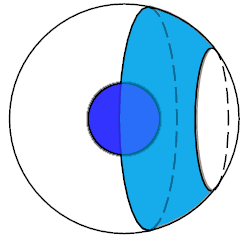
\includegraphics[width=0.2\textwidth]{content/4_3_autoNavigation/img/OrbitTransitionSphericalZone}
    \caption{Spherical zone of locations available for the interplanetary transition.}
    \label{fig:orbital-transition-zone}
\end{wrapfigure}

The transition for interplanetary movement is to move to the closest location in this spherical zone via orbital
movement, which results in a scene similar to the viewport in figure~\ref{fig:orbital-transition-angles}, where the
viewport is focused on the center of the origin's body, and the target body is within the $\alpha$ and $\beta$
margins in the viewport.

\subsubsection{Interplanetary Movement}\label{subsubsec:interplanetary-movement}

The interplanetary movement remains closest to the original movement.
However, the interpolation between the origin and target orientation is removed in order to separate rotation from
translation and increase predictability.
Instead, the rotation is split into an initial rotation to fave the traveling direction, so the user always moves
forward, towards the target, and a final rotation at the end of the translation to rotate the observer into the final
orientation at the target location.

The translation uses a straight spline.
This way the movement is similar to the original interpolation between the origin and target position.
However, the spline allows easier modification of the path, leading to easier collision detection and mitigation in
the future, since the spline can be easily checked for collisions and, if necessary, additional control points can be
inserted into the spline to avoid collisions.
The interplanetary movement always ends in either an interplanetary location (bookmark) or a target body's orbit,
where orbital movement can be resumed.
Therefore, no transition from interplanetary movement to orbital movement is needed.

\begin{figure}[h]
    \centering
    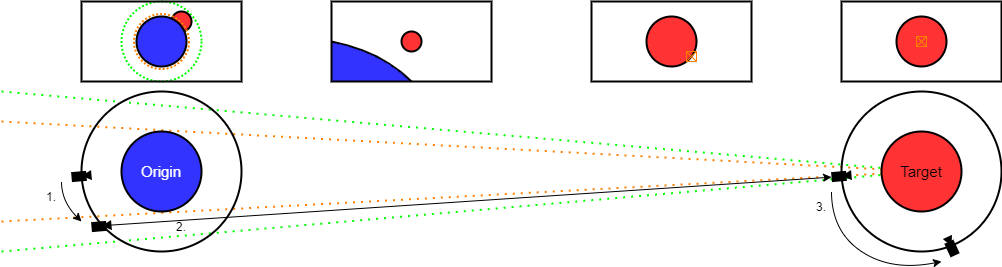
\includegraphics[width=\textwidth]{content/4_3_autoNavigation/img/Orbit2OrbitExample}
    \caption{Example of automatic movement including the orbital to interplanetary movement transition (1.), the
    interplanetary movement (2.), and orbital movement the the final position (3.).}
    \label{fig:orbital-example}
\end{figure}

An example of movement between two orbital locations, is shown in figure~\ref{fig:orbital-example}.
The first step shown in the figure is the transition from an arbitrary orbital location around the origin body to a
location that fulfills the requirements (equations~\ref{eq:orbital-angles}~\&~\ref{eq:orbital-magnitudes}).

The second step is the interplanetary movement between the origin orbit, and the target orbit.
First, the observer rotates from focusing on the origin's center to the target's center, and travel direction.
During this rotation the requirements for the transition between orbital and interplanetary movement, help reduce the
angular distance of the rotation and prevent collision with the origin body during interplanetary travel.

After arriving at the target's orbit, the third step is an orbital movement to the final position.

While this staged approach increases the overall travel time of the automatic navigation, we aim to reduce
disorientation and resulting cybersickness symptoms by providing the user with an easily predictable solution that
decouples rotation from translation and minimizes complex and surprising rotations.


\subsection{Automatic Movement Implementation}\label{subsec:automatic-movement-implementation}

The automatic movement for CosmoScout is organized in two distinct parts.
The first part is the \mintinline{c}{moveTo}-method, where the parameters of the movement are processed, and the second
part is the \mintinline{c}{updateMovementAnimation}-method which is called every frame, polling the state of the
movement based on the current time.

The old \mintinline{c}{moveTo}-method uses the information about the current position and orientation for the origin, as
well as the parameter information about the target location, and the duration of the movement to construct two
\mintinline{c}{AnimatedValue} objects.

An \mintinline{c}{AnimatedValue} object is consists of a start and end value, as well as a start and end time.
The object then provides a method to poll the value using time as the parameter, returning either the start or
end value, if the time is outside the timespan provided by the start and end time of the
\mintinline{c}{AnimatedValue}, or the method returns an interpolated value between the start and end values relative
to the point in time between the start and end time.

One \mintinline{c}{AnimatedValue} is used for the translation, interpolating between the origin
position, and the target position over the duration of the movement.
The other \mintinline{c}{AnimatedValue} is used for the rotation, interpolating between the origin orientation and the
target orientation over the duration of the movement.

After the \mintinline{c}{moveTo}-method has processed the available information into the two
\mintinline{c}{AnimatedValue} objects, the \mintinline{c}{mAnimationInProgress} flag is set.
While the flag is true, the \mintinline{c}{updateMovementAnimation}-method uses the current time at each frame to
poll the current position and orientation from the \mintinline{c}{AnimatedValue} objects, until the time is past the
end time of both end times.
Afterwards, the \mintinline{c}{updateMovementAnimation} resets the \mintinline{c}{mAnimationInProgress} flag to false.

Since the automatic movement can potentially be called from anywhere in CosmoScout, including plugins, we plan to
ensure backwards compatibility while changing the way the automatic movement is performed.
Therefore, the original \mintinline{c}{moveTo}-method's signature is kept and additional signatures are added as needed.
The original \mintinline{c}{moveTo}-method was an interpolation between the origin and target location leading to a
linear movement path from the origin to the target.
Since the interplanetary movement shows similar characteristics, the \mintinline{c}{moveTo}-method that contains the old
method signature is also used for interplanetary travel, and generally linear movements.

The first change to the method is replacing the \mintinline{c}{AnimatedValue} object for the interpolation of the
observers position with a linear spline between the origin and target position, and using the
\mintinline{c}{AnimatedValue} object to interpolate the $t$ parameter over the length of the spline relative to the
duration of the movement.

Second, split the rotation into an initial rotation, from the origin orientation to a \mintinline{c}{mLookAtPoint} in
movement direction, and a final rotation, from the \mintinline{c}{mLookAtPoint} to the final orientation.
Additionally, the rotations are separated from the translation by adjusting the start and end times of the
\mintinline{c}{AnimatedValue}-objects.

The overall duration ($t_{all}$) is split into three stages, the initial rotation ($t_{start}$), the translative phase
($t_{move}$), and the final rotation ($t_{end}$).
For the duration of each rotation a function (equation~\ref{eq:duration-weight}) is used that calculates a weight
factor ($w$) between 0 and 1 based on the angular difference ($\theta$) of the start and the end direction of view
(negative $z$-axis).
This way, the durations for each rotation can vary in length based on the angular difference of the rotation, and the
translative phase takes up the rest of the duration as described in the following equations:
\begin{equation}
    \label{eq:duration-timings}
    \frac{w_{start}}{3} t_{start} + (1 - \frac{w_{start}}{3} - \frac{w_{end}}{3}) t_{move} +
    \frac{w_{end}}{3} t_{end} = t_{all}
\end{equation}
with:
\begin{equation}
    \label{eq:duration-weight}
    w = f(\theta) = - \frac{\cos{\theta} - 1}{2}
\end{equation}
This results in the following limitations for the durations:
\begin{equation}
    \label{eq:duration-result-rot}
    0 \leq t_{start}, t_{end} \leq \tfrac{1}{3} t_{all}
\end{equation}
\begin{equation}
    \label{eq:duration-result-mov}
    \tfrac{1}{3} t_{all} \leq t_{move} \leq t_{all}
\end{equation}

The modifications to the \mintinline{c}{moveTo}-method also require changes to the
\mintinline{c}{updateMovementAnimation}-method, as the position and rotation needs to be polled from different sources.
Additionally, the simulation is changed to stop the simulation time during movement.
The automatic movement is programmed to transform all positions into the target's SPICE frame, and the delay of the
initial rotation before translation results in inadvertent movement, as the target frame rotates, moving the observer
significantly due to the distance to the target's center.

\subsubsection{Changes to \mintinline{c}{updateMovementAnimation}}\label{subsubsec:changes-to-updatemovementanimation}

\begin{minted}{c}
    void CelestialObserver::updateMovementAnimation(double tTime) {
        if (mAnimationInProgress) {
            // get position from spline
            mPosition = mMoveSpline->getPosition(mAnimatedT.get(tTime));

            if (tTime < mAnimatedRotationStart.mEndTime) {
                // rotation to look-at point not done yet
                mRotation = mAnimatedRotationStart.get(tTime);
            } else if (tTime > mAnimatedRotationFinal.mStartTime) {
                // rotation to final direction started
                mRotation = mAnimatedRotationFinal.get(tTime);
            } else {
                // observer is moving along spline -> adjust rotation towards look-at point
                auto direction = glm::normalize(mLookAtPoint - mPosition);
                mRotation      = glm::quatLookAt(direction, mUpDirection);
            }

            if (mAnimatedRotationFinal.mEndTime < tTime) {
                mAnimationInProgress = false;
                if (!mMovementQueue.empty()) {
                    moveTo(mMovementQueue.front());
                    mMovementQueue.pop();
                }
            }
        }
    }
\end{minted}
The polling of the current position only has minimal changes (l.\@4), as the \mintinline{c}{AnimatedValue}
is polled to receive the $t$ parameter for the position on the spline based on the current time, instead of receiving
the interpolated position directly from the \mintinline{c}{AnimatedValue}.

Polling the orientation is dependent on the current time in the movement process (ll.\@6--16).
If the current time is before the end time of the initial rotation, the current orientation is provided by the
\mintinline{c}{AnimatedValue} of the initial rotation, interpolating between the original orientation, and the
orientation towards the \mintinline{c}{mLookAtPoint}.
If the current time is after the start time of the final rotation, the orientation is provided by the
\mintinline{c}{AnimatedValue} of the final rotation, interpolating between the orientation aimed at the
\mintinline{c}{mLookAtPoint}, and the final orientation.
Otherwise, the movement animation is in the translative phase, and the current orientation is calculated using the 
\mintinline{c}{mLookAtPoint}, and the \mintinline{c}{mUpDirection} to generate a new orientation focused on the
\mintinline{c}{mLookAtPoint}.
The \mintinline{c}{mUpDirection} is saved from the orientation of the observer at the beginning of the movement
animation, to prevent the camera from any rolling rotations during the movement animation, since rolling during
movements appears to increase disorientation and therefore discomfort in users.
Lines 18--24 of the code block contain another important change that is explained in the next section.

\subsubsection{Movement description packages and Movement Queue}\label{subsubsec:movement-description-packages-and-movement-queue}

Based on the new changes to the \mintinline{c}{updateMovementAnimation}-method, there are the following requirements any
movement must fill with data in order for the movement animation to display correctly:
\begin{itemize}
    \item The \mintinline{c}{mMoveSpline}, providing the path for the movement, and the \mintinline{c}{AnimatedValue}
    for the interpolation of the $t$ parameter for the spline.
    \item The \mintinline{c}{AnimatedValue} for the initial rotation from the origin direction towards the
    \mintinline{c}{mLookAtPoint}.
    \item The \mintinline{c}{mLookAtPoint} to focus on during the translation, and the \mintinline{c}{mUpDirection}
    to calculate the orientation and prevent rolling.
    \item The \mintinline{c}{AnimatedValue} for the final rotation from the direction towards the
    \mintinline{c}{mLookAtPoint} to the final direction.
\end{itemize}
Any new movement must provide these information and therefore, a movement always consist of the initial rotation,
then the translation with a given point focused in the center of the viewport during the movement, and a final
rotation into the final orientation.

To provide functionality for the transitions, as well as future, potentially complex movements and routes, a queue is
added to the automatic movement system.
The parameters needed by the \mintinline{c}{moveTo}-methods to process into the above mentioned requirements are
packaged into structs, and the \mintinline{c}{mMovementQueue} provides a FIFO queue to hold an ordered list of these
movement instructions.
At the end of the \mintinline{c}{updateMovementAnimation}-method (ll.\@18--24), the
\mintinline{c}{mMovementQueue} is checked whether it contains any items, and if so, the topmost item is removed, and the
\mintinline{c}{moveTo}-method is called with the struct as parameter.
For this additional \mintinline{c}{moveTo}-methods can be added to provide different types of movement.
Additionally, a \mintinline{c}{moveTo}-method is added that accepts a queue of movement instructions as a parameter, as
shown below:
\begin{minted}{c}
    void CelestialObserver::moveTo(std::queue<MovementDescription> const& moveDescriptionsQueue) {
        // make sure queue contains at least one element
        if (!moveDescriptionsQueue.empty()) {
            // swap new movements into queue
            mMovementQueue = moveDescriptionsQueue;
            // execute first movement instruction
            moveTo(mMovementQueue.front());
            mMovementQueue.pop();
        }
    }
\end{minted}
Providing a new, non-empty queue to the method during an ongoing movement discards remaining items, emplaces the
new queue into the \mintinline{c}{mMovementQueue}, and calls the \mintinline{c}{moveTo}-method with the topmost item
of the queue.
Discarding the old queue when receiving a new queue is done, to prevent buffering of multiple, potentially unwanted
movements.

\begin{figure}[h]
    \centering
    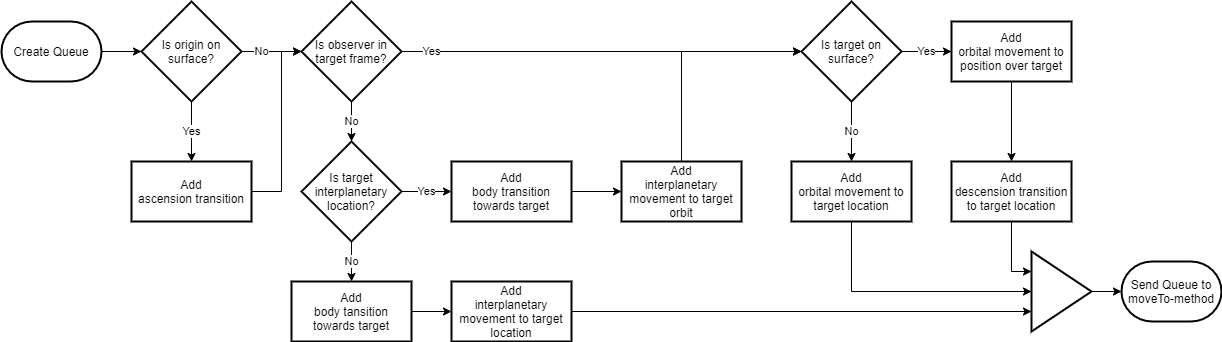
\includegraphics[width=\textwidth]{content/4_3_autoNavigation/img/QueueConstructionFlowchart}
    \caption{Flowchart for the construction of a movement queue.}
    \label{fig:movement-queue}
\end{figure}

Currently, the \mintinline{c}{mMovementQueue} can be filled with a variant of the two basic movement description
packages.
Either the linear movement that resulted from the original \mintinline{c}{moveTo}-method, and is used in the
interplanetary movement, or the circular movement that is used in the orbital movement.
The construction of a movement queue based on information about origin and target location is shown in the
flowchart in figure~\ref{fig:movement-queue}.

\subsubsection{Different \mintinline{c}{moveTo}-methods and control point computation}\label{subsubsec:different-moveto-methods-and-control-point-computation}

To provide different types of movement, the \mintinline{c}{moveTo}-method has multiple implementation with different
signatures:
\begin{minted}{c}
    void moveTo(std::string const& centerName, std::string const& frameName,
        glm::dvec3 const& position, glm::dquat const& rotation, double simulationTime,
        double realStartTime, double realEndTime);

    [...]

    void moveTo(DefaultPoint2Point const& moveDescriptionP2P);

    [...]

    void moveTo(DefaultOrbit const& moveDescriptionOrbit);

    [...]

    void moveTo(MovementDescription const& moveDescription);

    [...]

    void moveTo(std::queue<MovementDescription> const& moveDescriptionsQueue);
\end{minted}
The original signature of the method (l.\@1) is kept to allow backwards compatibility.
The second signature (l.\@7) accepts movement description packages for linear, point-to-point (interplanetary)
movements.
The function simply unpacks and relays the parameters for the linear movement to the first \mintinline{c}{moveTo}-method.
The third signature (l.\@11) accepts movement description packages for circular (orbital) movements.
The fourth signature (l.\@15) is added because the movement queue uses a variant type for its elements.
Therefore, when a new element for the queue is used, this method accepts it.
The method checks the real movement description type using a switch-case-statement, and typecasts the variant-type
elements, and relays them to their respective methods.
The last signature (l.\@19) accepts whole movement queues to be passed and is described above.
Currently, only linear and circular movement packages are implemented, however, the addition of further movement
description packages is straightforward in this system.

The movement path is constructed using a uniform cubic basis splines.
Uniform cubic b-splines offer some advantages over other curves, as they are similar to bezier curves, which means
they are relatively easy to construct, and have a continuous velocity over the curve.
Additionally, uniform cubic b-splines offer a continuous curvature, easing the movement of the observer along the
spline.
Lastly, their control points only have local influence on the curve, which means that additional control points can
be inserted to handle collisions, without major changes to the overall curve.
Their only disadvantage, the interpolated curve not necessarily passing through the specified control points, can be
mitigated by inserting triplets of control points with the middle point being the control point teh curve should pass
close to, and the other two points representing a tangent to the curve that is passing through the three control points.

Uniform cubic b-splines that are non-looping also require an additional point on either end of the curve where the
curve is not interpolated.
Therefore, the curve for the movement always starts in the second and ends in the penultimate control point.

The spline for the interplanetary movement is constructed between the origin and target using two triplets of control
points.

\begin{figure}[h]
    \centering
    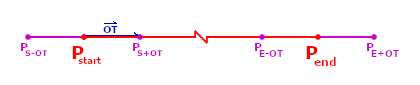
\includegraphics[width=0.5\textwidth]{content/4_3_autoNavigation/img/LinearSplinePoints}
    \caption{Control points of a linear spline with the start and end point ($P_{start}$, $P_{end}$), and the control
    points ($P_{S-OT}$, $P_{S+OT}$, $P_{E-OT}$, $P_{E+OT}$) making up each triplet.}
    \label{fig:linear-control-points}
\end{figure}

First, the vector between the origin and target ($OT$-vector) is constructed and normalized.
Then, each triplet forms the tangent through the start and end point, where the start or end point is the middle
control point, with one control point in front, and one control point behind the middle point in direction of the
$OT$-vector, as described in figure~\ref{fig:linear-control-points}.
This way, bot the tangent in the start and end point are along the $OT$-vector, leading to a straight spline between
the start and end point.
The resulting spline is saved in the \mintinline{c}{mMoveSpline}, and the \mintinline{c}{AnimatedValue}-object for the
interpolation of the $t$ parameter is set to interpolate between $0$ and $t_{max}$ ($1$ in most cases) over the
duration of the translation phase.

The \mintinline{c}{mLookAtPoint} is set to the last control point, as it is slightly in front of the end point of the
interpolated spline.
This way the observer is always oriented towards the end point of the movement path, without the movement ending in a
location where the position and \mintinline{c}{mLookAtPoint} coincide, which could lead to an undefined orientation
for the observer.
Additionally, the \mintinline{c}{mUpDirection} is saved from the up-direction of the observer in the origin location to
prevent the observer from rolling during the movement phase.

Finally, the \mintinline{c}{AnimatedValue}-objects for the initial, and the final rotation are set.
The initial rotation interpolates between the origin orientation, and the orientation towards the
\mintinline{c}{mLookAtPoint} over the duration for the initial rotation.
The final rotation interpolates between the orientation towards the \mintinline{c}{mLookAtPoint} and the final
orientation over the duration for the final rotation.

The durations and points in time for the rotations and the translation are calculated as mentioned above
(equations~\ref{eq:duration-weight}~and~\ref{eq:duration-timings}).

The orbital movement uses a different \mintinline{c}{moveTo}-method to realize the circular movement path.
To approximate the circular arc between the start and end point, both points are projected into 2D space by finding
the normal to the plane defined by the center-start, and center-end vectors ($\overrightarrow{cs}$ and
$\overrightarrow{ce}$).
This also results in the shortest possible path in orbit from the start to the end point.
Next, the angle ($\theta$) between the two vectors is calculated, and both vectors are normalized to compute the
additional control points on the unit circle.

\begin{figure}[h]
    \centering
    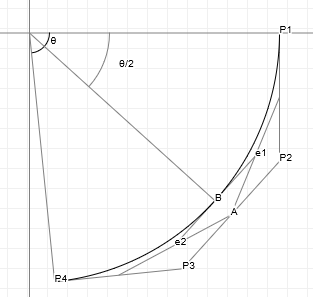
\includegraphics[width=0.5\textwidth]{content/4_3_autoNavigation/img/CircularCurveParameters}
    \caption{Control points ($P2$, $P3$), the start point ($P1$), end point ($P4$) and angle ($\theta$) in 2D
    space~\cite{Poxmax2021}.}
    \label{fig:orbital-control-points}
\end{figure}

Figure~\ref{fig:orbital-control-points} shows an example of the transformation into 2D space, and the required
control points ($P1$, $P2$, $P3$, and $P4$).
Poxmax~\cite{Poxmax2021} derived a formula to calculate the missing control points $P2$ and $P3$ on the unit circle:
\begin{equation}
    \label{eq:control-points}
    \begin{aligned}
        P_{start} &= P1 = (1, 0) \\
        P_{c1} &= P2 = (1, k) \\
        P_{c2} &= P3 = (\cos(\theta) + k \cdot \sin(\theta), \sin(\theta) - k \cdot \cos(\theta)) \\
        P_{end} &= P4 = (\cos(\theta), \sin(\theta))
    \end{aligned}
\end{equation}
With:
\begin{equation}
    \label{eq:control-points-factor}
    \begin{aligned}
        k &= f(\theta) = \frac{4}{3} \cdot \tan\left( \frac{\theta}{4} \right)
    \end{aligned}
\end{equation}
To transform the control points back into 3D space, the oriented angle around the center from $P1$ to $P2$
($\phi_{start}$), and from $P4$ to $P3$ ($\phi_{end}$) is calculated.
To get the control points, the start position and end position are rotated around the normal of the 2D plane, and
scaled by the magnitude of their 2D counterpart.

\begin{figure}[h]
    \centering
    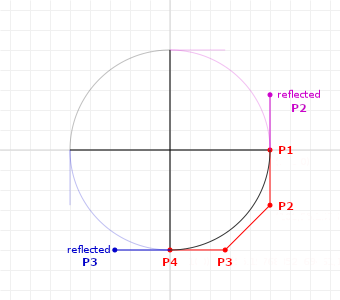
\includegraphics[width=0.5\textwidth]{content/4_3_autoNavigation/img/ControlPointsReflected}
    \caption{Example control points for circular spline where $\theta = 90\deg$~\cite{Poxmax2021}.}
    \label{fig:orbital-reflected-points}
\end{figure}

Since, the spline needs two additional control points where the spline is not interpolated, the calculated control
points are also reflected to the other side of the start and end position as shown in
figure~\ref{fig:orbital-reflected-points}.

The control points in 3D space ($C_{P2}$, $C_{P3}$), and their reflections ($C_{rP2}$, $C_{rP3}$) can be calculated
using Rodrigues' rotation formula with the start and end points ($C_{start}$, $C_{end}$), the normal for the 2D plane
($\vec{N}$), the angles between the control point, and the start, or end point ($\phi_{start}$, $\phi_{end}$), and the
control points in 2D space ($\overrightarrow{P2}$, $\overrightarrow{P3}$):
\begin{equation}
    \label{eq:control-point-transformation}
    \begin{aligned}
        \vec{C}_{P2} &= \left(
            \vec{C}_{start} \cos(\phi_{start}) +
            ( \vec{N} \times \vec{C}_{start} )\sin(\phi_{start}) +
            \vec{N} ( \vec{N} \cdot \vec{C}_{start} )( 1 - \cos(\phi_{start}) )
        \right) \cdot \left\| \overrightarrow{P2} \right\|
        \\
        \vec{C}_{rP2} &= \vec{C}_{start} - \left( \overrightarrow{C_{start}C_{P2}} \right) =
        2\vec{C}_{start} - \vec{C}_{P2}
        \\
        \vec{C}_{P3} &= \left(
            \vec{C}_{end} \cos(\phi_{end}) +
            ( \vec{N} \times \vec{C}_{end} )\sin(\phi_{end}) +
            \vec{N} ( \vec{N} \cdot \vec{C}_{end} )( 1 - \cos(\phi_{end}) )
        \right) \cdot \left\| \overrightarrow{P3} \right\|
        \\
        \vec{C}_{rP3} &= \vec{C}_{end} - \left( \overrightarrow{C_{end}C_{P3}} \right) =
        2\vec{C}_{end} - \vec{C}_{P3}
    \end{aligned}
\end{equation}
Since the start and end position are used to derive the adjacent control points, different orbit heights in start and
end position are carried over to their adjacent control points, keeping the triplet of control points on the tangent
to the movement curve in the start or end position.
Differences in orbit height between the start triplet and end triplet lead to the movement spline becoming more
elliptical, resulting in a zoom effect from the start to the end orbit height during the rotation around the center.

With the control points calculated, the \mintinline{c}{mMoveSpline} can be constructed, and the
\mintinline{c}{AnimatedValue}-object for the $t$ parameter can be set to interpolate the position along the spline
over the duration of the movement phase.
The \mintinline{c}{mLookAtPoint} for the orientation during the translation phase is set to the center of the body,
and the \mintinline{c}{mUpDirection} is saved from the origin orientation to prevent rolling during the movement.
The \mintinline{c}{AnimatedValue}-object for the initial rotation is set to interpolate from the origin orientation
to the orientation facing the center of the body over the duration of the initial rotation.
The \mintinline{c}{AnimatedValue}-object for the final rotation is set to interpolate from the orientation facing the
center of the body to the final orientation over the duration of the final rotation.
The durations for the two rotation are calculated in the same way as the durations for the linear movement, based on
the angular difference between the start and end direction.
However, to properly calculate the angular difference, roll rotation has to be taken into account as well, therefore
the difference between the start and end quaternion is used to calculate the weight instead of the
equation~\ref{eq:duration-weight}.
